\begin{figure}[htbp]
\centering
\resizebox{\textwidth}{!}{%
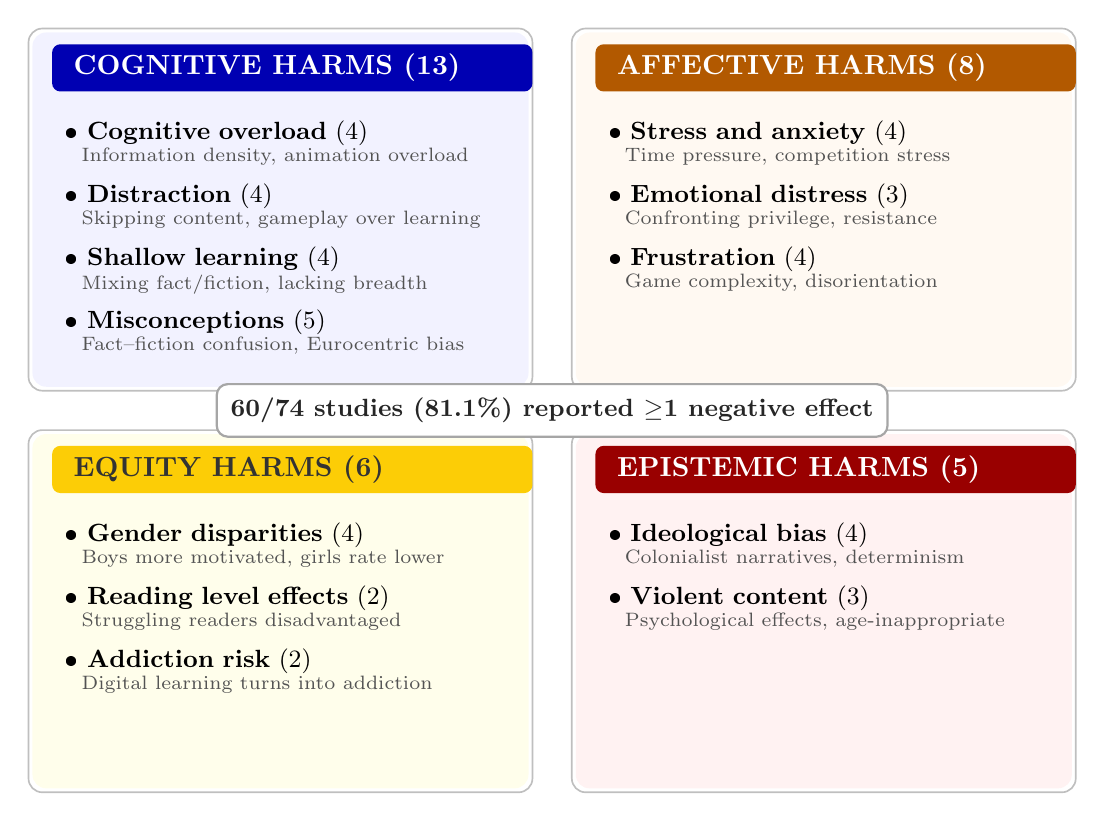
\begin{tikzpicture}[
  subcat/.style={font=\small, anchor=north west, text width=5.6cm},
  example/.style={font=\scriptsize, text=gray!65!black, anchor=north west, text width=5.4cm},
]

% Quadrant dimensions
\def\qw{6.4}     % quadrant inner width
\def\qh{4.6}     % quadrant inner height
\def\gap{0.5}     % gap between quadrants
\def\hw{6.4}      % header bar width

% Derived positions
\pgfmathsetmacro{\rx}{\qw + \gap}        % right column x
\pgfmathsetmacro{\by}{-\qh - \gap}       % bottom row y
\pgfmathsetmacro{\cx}{(\qw + \gap/2)}    % center x
\pgfmathsetmacro{\cy}{(-\qh - \gap/2)}   % center y

% ============================================================
% QUADRANT 1: COGNITIVE HARMS (top-left)
% ============================================================
\draw[gray!50, rounded corners=5pt, line width=0.6pt]
  (0, 0) rectangle (\qw, -\qh);
\fill[blue!5, rounded corners=5pt]
  (0.05, -0.05) rectangle (\qw-0.05, -\qh+0.05);

\fill[blue!70!black, rounded corners=3pt]
  (0.3, -0.2) rectangle (\hw, -0.8);
\node[font=\normalsize\bfseries, text=white, anchor=west]
  at (0.45, -0.5) {COGNITIVE HARMS (13)};

\node[subcat] at (0.35, -1.05) {%
  \textbullet~\textbf{Cognitive overload} (4)};
\node[example] at (0.55, -1.40) {%
  Information density, animation overload};
\node[subcat] at (0.35, -1.85) {%
  \textbullet~\textbf{Distraction} (4)};
\node[example] at (0.55, -2.20) {%
  Skipping content, gameplay over learning};
\node[subcat] at (0.35, -2.65) {%
  \textbullet~\textbf{Shallow learning} (4)};
\node[example] at (0.55, -3.00) {%
  Mixing fact/fiction, lacking breadth};
\node[subcat] at (0.35, -3.45) {%
  \textbullet~\textbf{Misconceptions} (5)};
\node[example] at (0.55, -3.80) {%
  Fact--fiction confusion, Eurocentric bias};

% ============================================================
% QUADRANT 2: AFFECTIVE HARMS (top-right)
% ============================================================
\draw[gray!50, rounded corners=5pt, line width=0.6pt]
  (\rx, 0) rectangle (\rx+\qw, -\qh);
\fill[orange!5, rounded corners=5pt]
  (\rx+0.05, -0.05) rectangle (\rx+\qw-0.05, -\qh+0.05);

\fill[orange!70!black, rounded corners=3pt]
  (\rx+0.3, -0.2) rectangle (\rx+\hw, -0.8);
\node[font=\normalsize\bfseries, text=white, anchor=west]
  at (\rx+0.45, -0.5) {AFFECTIVE HARMS (8)};

\node[subcat] at (\rx+0.35, -1.05) {%
  \textbullet~\textbf{Stress and anxiety} (4)};
\node[example] at (\rx+0.55, -1.40) {%
  Time pressure, competition stress};
\node[subcat] at (\rx+0.35, -1.85) {%
  \textbullet~\textbf{Emotional distress} (3)};
\node[example] at (\rx+0.55, -2.20) {%
  Confronting privilege, resistance};
\node[subcat] at (\rx+0.35, -2.65) {%
  \textbullet~\textbf{Frustration} (4)};
\node[example] at (\rx+0.55, -3.00) {%
  Game complexity, disorientation};

% ============================================================
% QUADRANT 3: EQUITY HARMS (bottom-left)
% ============================================================
\draw[gray!50, rounded corners=5pt, line width=0.6pt]
  (0, \by) rectangle (\qw, \by-\qh);
\fill[yellow!8, rounded corners=5pt]
  (0.05, \by-0.05) rectangle (\qw-0.05, \by-\qh+0.05);

\fill[yellow!65!orange, rounded corners=3pt]
  (0.3, \by-0.2) rectangle (\hw, \by-0.8);
\node[font=\normalsize\bfseries, text=black!80, anchor=west]
  at (0.45, \by-0.5) {EQUITY HARMS (6)};

\node[subcat] at (0.35, \by-1.05) {%
  \textbullet~\textbf{Gender disparities} (4)};
\node[example] at (0.55, \by-1.40) {%
  Boys more motivated, girls rate lower};
\node[subcat] at (0.35, \by-1.85) {%
  \textbullet~\textbf{Reading level effects} (2)};
\node[example] at (0.55, \by-2.20) {%
  Struggling readers disadvantaged};
\node[subcat] at (0.35, \by-2.65) {%
  \textbullet~\textbf{Addiction risk} (2)};
\node[example] at (0.55, \by-3.00) {%
  Digital learning turns into addiction};

% ============================================================
% QUADRANT 4: EPISTEMIC HARMS (bottom-right)
% ============================================================
\draw[gray!50, rounded corners=5pt, line width=0.6pt]
  (\rx, \by) rectangle (\rx+\qw, \by-\qh);
\fill[red!5, rounded corners=5pt]
  (\rx+0.05, \by-0.05) rectangle (\rx+\qw-0.05, \by-\qh+0.05);

\fill[red!60!black, rounded corners=3pt]
  (\rx+0.3, \by-0.2) rectangle (\rx+\hw, \by-0.8);
\node[font=\normalsize\bfseries, text=white, anchor=west]
  at (\rx+0.45, \by-0.5) {EPISTEMIC HARMS (5)};

\node[subcat] at (\rx+0.35, \by-1.05) {%
  \textbullet~\textbf{Ideological bias} (4)};
\node[example] at (\rx+0.55, \by-1.40) {%
  Colonialist narratives, determinism};
\node[subcat] at (\rx+0.35, \by-1.85) {%
  \textbullet~\textbf{Violent content} (3)};
\node[example] at (\rx+0.55, \by-2.20) {%
  Psychological effects, age-inappropriate};

% ============================================================
% CENTER ANNOTATION
% ============================================================
\node[draw=gray!70, fill=white, rounded corners=4pt,
    font=\small\bfseries, text=gray!30!black, inner sep=5pt,
    line width=0.8pt]
    at (\cx, \cy)
    {60/74 studies (81.1\%) reported $\geq$1 negative effect};

\end{tikzpicture}%
}% end resizebox
\caption{Harm landscape of gamification in history education. Negative effects from the 74-study corpus are systematised into four categories: cognitive, affective, equity, and epistemic harms. Numbers indicate studies reporting each subcategory; 60 of 74 studies (81.1\%) reported at least one negative effect.}
\label{fig:harm-landscape}
\end{figure}
